\documentclass[12pt]{article}

% Template oficial da SBC (sbc-template.sty e sbc.bst, baixados de sbc.org.br), sem alterações de margens,
% fontes, espaçamento ou número de colunas.
\usepackage{sbc-template}
\usepackage{graphicx,url}
\usepackage[utf8]{inputenc}
\usepackage[T1]{fontenc}
\usepackage[brazilian]{babel}
\usepackage{tikz}
\usetikzlibrary{positioning,arrows.meta}

\graphicspath{{figuras/}{../figuras/}}

\sloppy

\title{Sinaliza: aprendizado de máquina para decidir quais palavras\\
de um texto em português viram sinais de Libras}

\author{Amanda Montarroyos\inst{1}, Bruno Assunção\inst{1}, Caio Ferreira\inst{1},\\
  Carlos Eduardo\inst{1}, Fabiana Coelho\inst{1}, Felipe Marques\inst{1}}

\address{CESAR School -- Recife -- PE -- Brasil\email{\{amo,bas,cflo,ceec,fcsls,fmmo\}@cesar.school}}

\begin{document}

\maketitle

\begin{abstract}
  Sinaliza receives a text in Brazilian Portuguese and plays the corresponding sequence of Libras
  signs on an avatar. Its machine learning component is a word-level binary classifier, trained on
  the VLibrasBD corpus (127 thousand sentences glossed by certified interpreters), that decides whether
  each word becomes a sign. We compared Logistic Regression, Decision Tree, Random Forest and KNN,
  tuned the Random Forest with Optuna and validated it with sentence-grouped cross-validation. On a
  held-out test set used once, it reached macro-F1 of 0.885 against 0.823 for the fixed stop-word list
  previously used. The solution runs with Airflow, MLflow, an API, a simulated embedded device
  publishing over MQTT and a dashboard, all started by a single Docker Compose command.
\end{abstract}

\begin{resumo}
  O Sinaliza recebe um texto em português e toca, num avatar, a sequência de sinais de Libras
  correspondente. O aprendizado de máquina está num classificador binário por palavra, treinado no
  corpus VLibrasBD (127 mil frases glosadas por intérpretes certificados), que decide se cada palavra
  vira sinal. Comparamos Regressão Logística, Árvore de Decisão, Random Forest e KNN, otimizamos o
  Random Forest com Optuna e o validamos com validação cruzada agrupada por frase. No conjunto de teste,
  usado uma única vez, ele chegou a F1-macro de 0,885, contra 0,823 da lista fixa usada antes. A solução
  roda com Airflow, MLflow, API, um sistema embarcado simulado que publica via MQTT e um painel, tudo
  com um único comando do Docker Compose.
\end{resumo}

\section{Introdução}

A Língua Brasileira de Sinais (Libras) é a língua de boa parte da comunidade surda do Brasil, mas
serviços de atendimento raramente têm intérprete. Ferramentas como a Suíte VLibras~\cite{vlibras:26}
mostram, num avatar, sinais correspondentes a um texto em português. O Sinaliza, projeto do Grupo 10
nas disciplinas de Projetos 6 e de Aprendizado de Máquina da CESAR School, segue a mesma ideia: recebe
um texto e toca a sequência de sinais no player do VLibras.

Entre o texto e os sinais há uma decisão que um intérprete toma sem pensar: \emph{quais palavras viram
sinal}. Artigos, preposições e verbos de ligação costumam desaparecer na glosa; substantivos, verbos e
adjetivos ficam. Antes deste trabalho, o Sinaliza tomava essa decisão com uma lista fixa de 95 palavras
funcionais. Este relatório descreve a tarefa de aprendizado de máquina que substituiu essa lista, que
chamamos de \textbf{T1}: classificar cada palavra como \texttt{MANTER} (vira sinal) ou
\texttt{DESCARTAR}, aprendendo com as glosas feitas por intérpretes certificados no corpus
VLibrasBD~\cite{lima:25}.

Duas ressalvas valem para todo o texto. Primeiro, a saída do Sinaliza é uma \emph{sequência de sinais},
não uma tradução para Libras: não há gramática da Libras, ordem própria dos sinais nem expressão facial.
Segundo, ninguém da equipe sabe Libras; as métricas medem proximidade às glosas dos intérpretes, não
correção linguística nem aprovação de pessoas surdas.

O restante do relatório segue os blocos de avaliação da disciplina: dados e análise exploratória
(Seção~\ref{sec:dados}), metodologia de validação (Seção~\ref{sec:validacao}), modelagem e resultados
(Seção~\ref{sec:modelagem}), arquitetura e MLOps (Seção~\ref{sec:mlops}), limitações
(Seção~\ref{sec:limitacoes}) e conclusão (Seção~\ref{sec:conclusao}). O código, os notebooks e a
documentação estão em \url{https://github.com/Carlosesposito22/Sinaliza}.

\section{Dados e análise exploratória}\label{sec:dados}

\subsection{Base de dados e rotulagem}

O conjunto de dados inicial (\emph{bootstrap dataset}) é o VLibrasBD~\cite{lima:25}: 127.349 pares
de frase em português e glosa em Libras, escritos por intérpretes certificados, de dois domínios
(textos gerais e textos do portal gov.br). A ingestão baixa o arquivo, confere o SHA-256 publicado e
carrega a tabela \texttt{corpus\_bruto} no PostgreSQL.

A limpeza remove frases vazias, duplicatas exatas e glosas sem nenhum sinal, restando 127.320 pares.
Cada frase passa pelo spaCy~\cite{honnibal:20}, que dá lema, classe gramatical (UPOS), relação de
dependência e morfologia de cada palavra; a pontuação é retirada. O rótulo de cada palavra vem de uma
regra de alinhamento: \texttt{MANTER} se o lema ou a forma escrita aparece entre os sinais da glosa,
normalizada pela notação do corpus (por exemplo, \texttt{NÃO\_X} conta como \texttt{NÃO} e
\texttt{X}, e \texttt{1S\_X\_2S}, verbo direcional, conta como \texttt{X}). O resultado são
1.615.265 palavras rotuladas, 52,5\% delas \texttt{MANTER}.

Os atributos de cada palavra são 13 categóricos (classe gramatical, dependência, oito traços de
morfologia, tipo de frase e as classes das palavras anterior e seguinte), 4 numéricos (posição
absoluta e relativa, tamanho da frase e se é \emph{stopword}) e o lema. O encoding é \emph{one-hot}
para os categóricos e para os 2.000 lemas mais frequentes (os demais viram uma categoria
``infrequente''); os numéricos são padronizados quando o modelo é sensível à escala.

\textbf{Valores ausentes.} Não há células vazias. Os únicos ``ausentes'' são traços de morfologia que
não se aplicam (um substantivo não tem tempo verbal), presentes em 26\% (número) a 99\% (polaridade) das
palavras. Em vez de imputar, gravamos o valor como uma categoria própria, porque a ausência é
informativa: quando o tipo de pronome está presente (pronomes e artigos), só 18\% das palavras são
mantidas; quando falta, 62\%.

\subsection{Estatísticas descritivas}

As frases têm mediana de 7 palavras e média de 12,7 (desvio-padrão 13,1, assimetria 2,8, máximo 262);
a cauda longa justificou usar mediana e quartis nas análises. A glosa tem em média 64\% das palavras
da frase (desvio 0,17), com a mesma compressão nos dois domínios, embora as frases do gov.br sejam
mais longas (mediana de 11 palavras, contra 5). Há 17 classes gramaticais e 62.133 lemas distintos; os
dois domínios compartilham só 20,5\% do vocabulário, o que motivou o teste fora do domínio da
Seção~\ref{sec:validacao}.

\subsection{Visualizações}

O notebook de análise exploratória tem nove visualizações interpretadas; as quatro mais importantes
para a modelagem estão nas Figuras~\ref{fig:upos} a~\ref{fig:lemas}.

\begin{figure}[ht]
\centering
\begin{minipage}{.48\textwidth}\centering
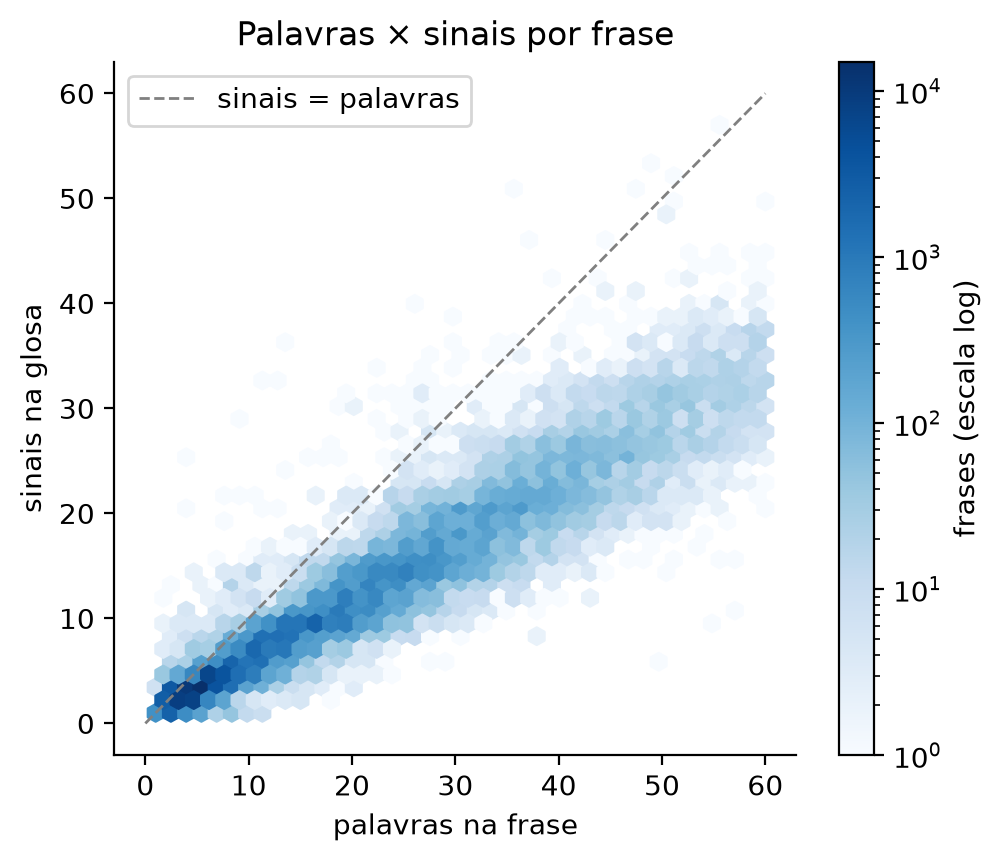
\includegraphics[width=\textwidth]{eda-02-palavras-x-sinais.png}
\end{minipage}\hfill
\begin{minipage}{.48\textwidth}\centering
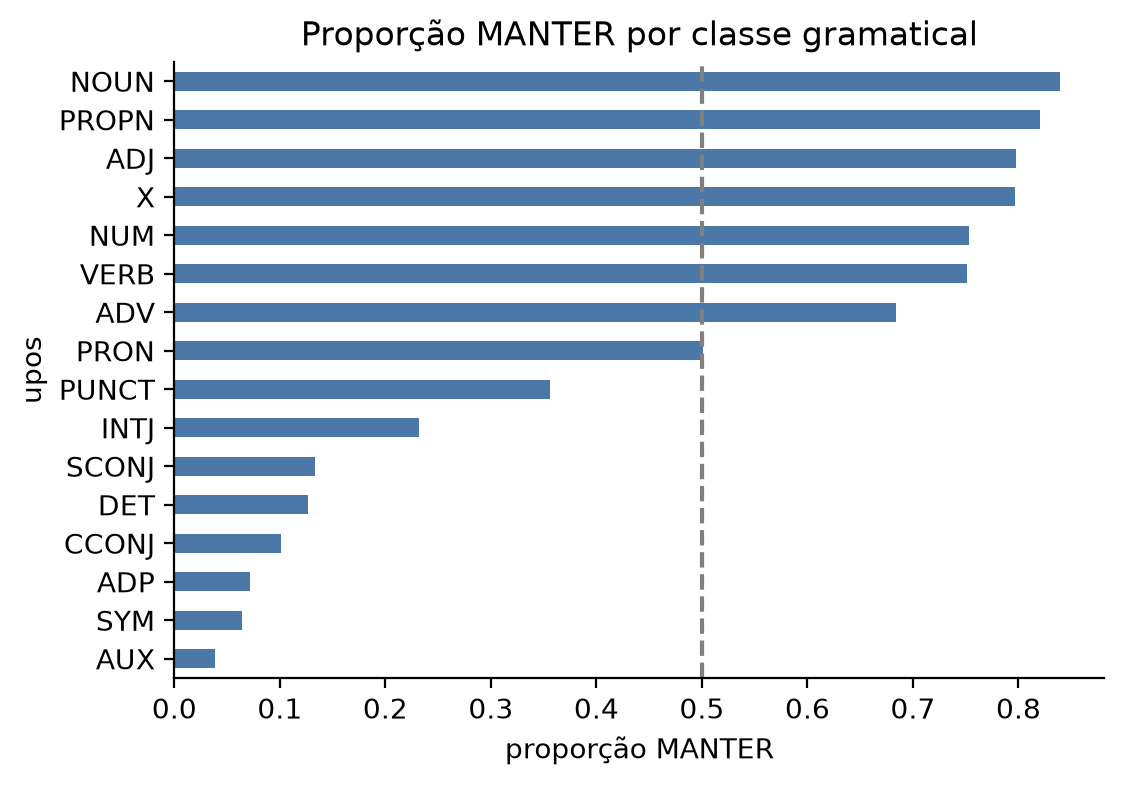
\includegraphics[width=\textwidth]{eda-05-upos.png}
\end{minipage}
\caption{À esquerda, palavras por frase contra sinais por glosa (escala logarítmica de frases): a glosa
cresce com a frase, mas fica sempre abaixo da diagonal. À direita, proporção de \texttt{MANTER} por
classe gramatical.}
\label{fig:upos}
\end{figure}

A Figura~\ref{fig:upos} mostra que o descarte não é uma taxa fixa por frase (a dispersão cresce com o
tamanho, correlação de Pearson 0,97) e que a classe gramatical separa bem os extremos: auxiliares,
preposições e artigos são mantidos em 4\% a 13\% das vezes; substantivos, nomes próprios e adjetivos,
em 80\% a 84\%. As classes do meio (pronomes, advérbios, verbos, numerais) são onde uma lista fixa erra.

\begin{figure}[ht]
\centering
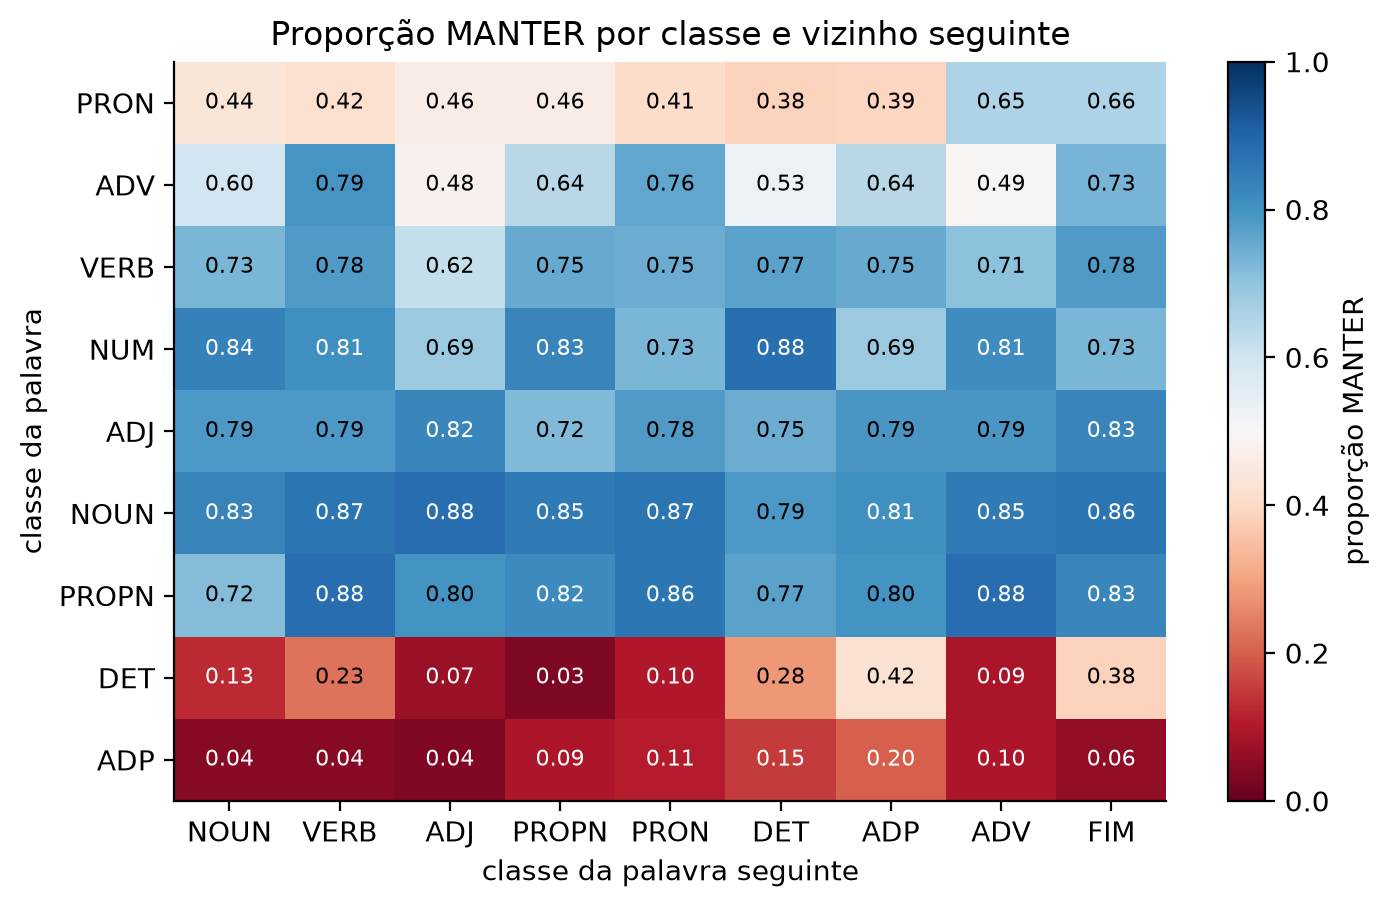
\includegraphics[width=.78\textwidth]{eda-06-contexto-vizinho.png}
\caption{Proporção de \texttt{MANTER} por classe da palavra e classe da palavra seguinte.}
\label{fig:contexto}
\end{figure}

A Figura~\ref{fig:contexto} justifica usar o contexto como atributo: o vizinho seguinte muda a
decisão das classes intermediárias. Um artigo é mantido em 3\% dos casos antes de nome próprio e em
42\% antes de preposição; um advérbio, em 48\% antes de adjetivo e 79\% antes de verbo. Substantivos,
adjetivos e nomes próprios ficam altos qualquer que seja o vizinho.

\begin{figure}[ht]
\centering
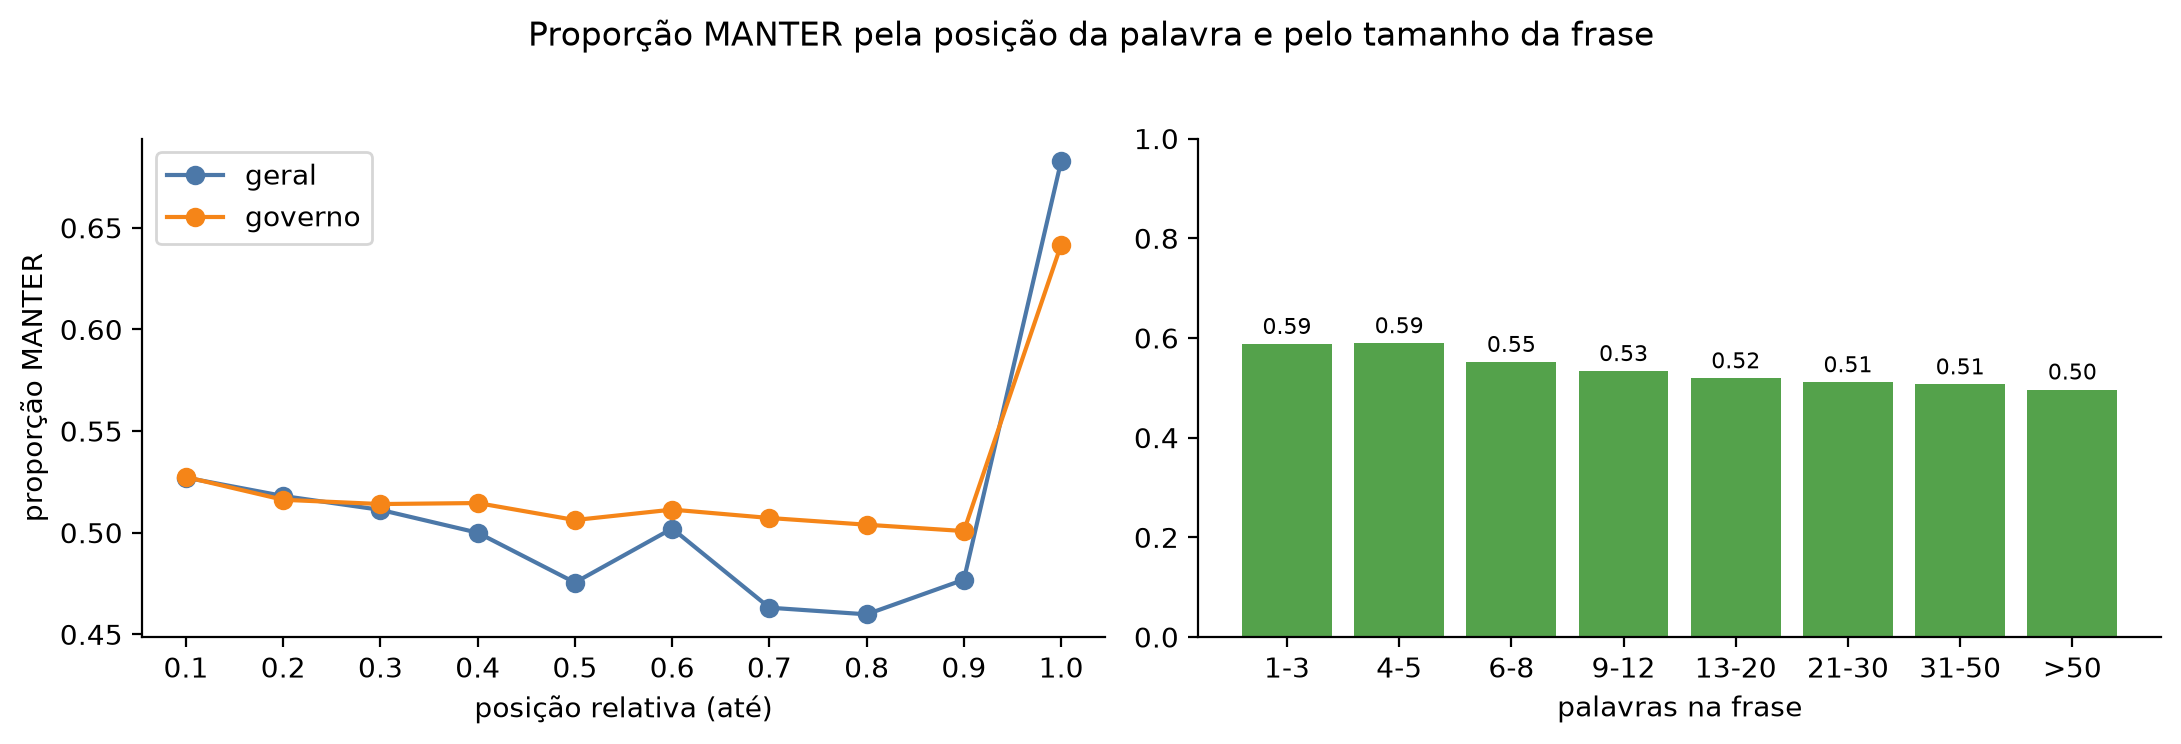
\includegraphics[width=\textwidth]{eda-07-posicao-tamanho.png}\\[4pt]
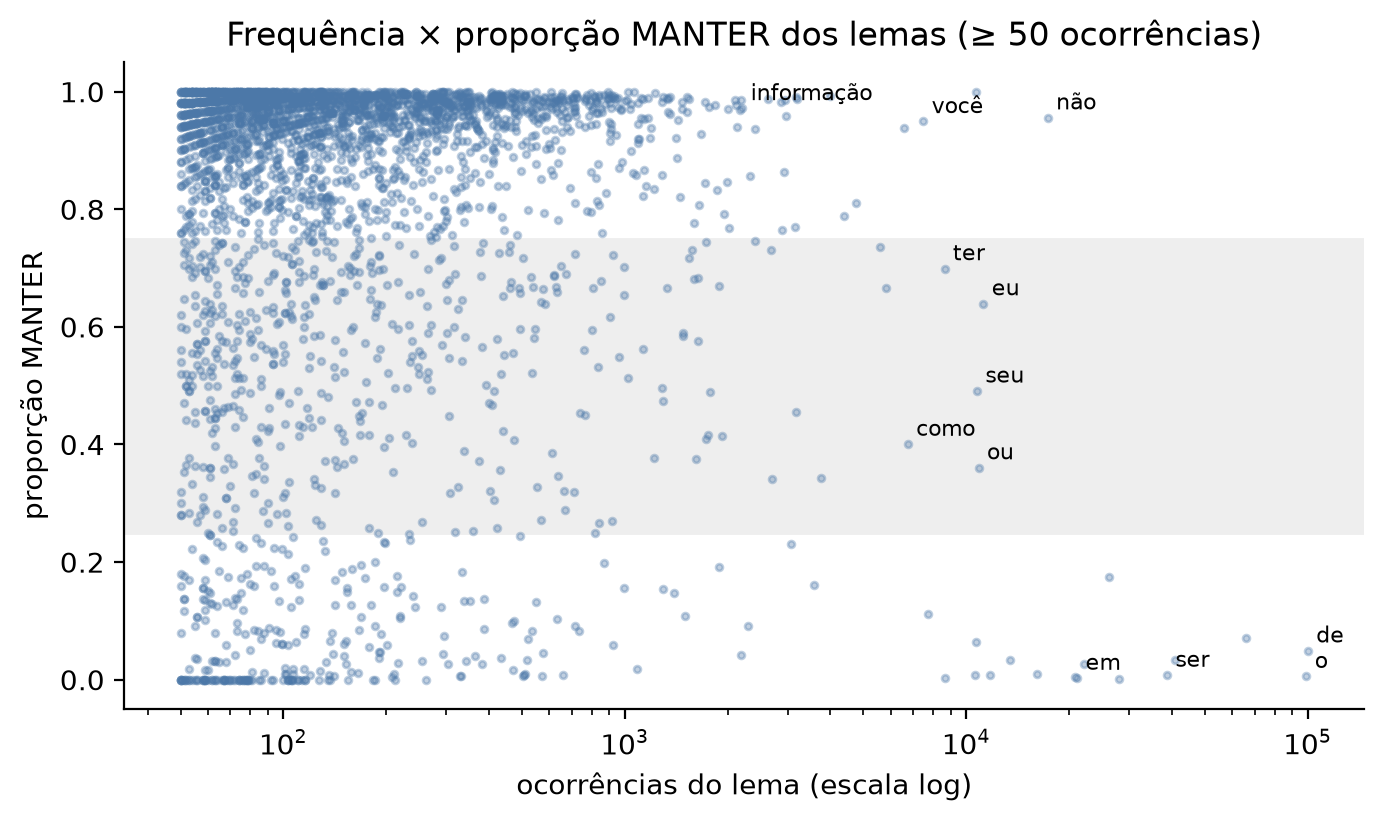
\includegraphics[width=.8\textwidth]{eda-08-lemas-ambiguos.png}
\caption{Acima, proporção de \texttt{MANTER} pela posição relativa na frase e pelo tamanho da
frase. Abaixo, frequência e proporção de \texttt{MANTER} de cada lema com 50 ou mais ocorrências; a
faixa cinza marca os lemas ambíguos.}
\label{fig:lemas}
\end{figure}

Na Figura~\ref{fig:lemas}, a proporção de \texttt{MANTER} sobe no último décimo da frase (0,64 a
0,68), onde costuma estar o núcleo, e cai devagar com o tamanho da frase; o efeito existe, mas é
fraco perto do da classe gramatical. Já os lemas ambíguos (entre 25\% e 75\% de \texttt{MANTER}) são
16,2\% dos lemas frequentes e 13,7\% das ocorrências, entre eles palavras muito comuns como ``eu'',
``seu'', ``ter'' e ``como''. Nesses casos qualquer lista fixa erra uma parte das ocorrências; é onde o
classificador, olhando o contexto, pode ganhar.

\subsection{Qualidade dos rótulos}

Como o rótulo vem de uma regra, a equipe conferiu à mão uma amostra de 200 palavras (100 de cada
classe), perguntando se a palavra, ou algo de mesmo sentido, aparece na glosa. O rótulo
\texttt{MANTER} errou em 1\% dos casos (intervalo de Wilson de 95\%: 0,2\% a 5,4\%) e o
\texttt{DESCARTAR} em 16\% (10,1\% a 24,4\%). Ponderando pela proporção real das classes, a taxa geral
de rótulos errados é de 8,1\% (4,6\% a 11,7\%). Os erros de \texttt{DESCARTAR} são palavras que o
intérprete manteve com outra forma: derivação (``melhoria'' e \texttt{MELHORAR}), sinônimo
(``solicitar'' e \texttt{PEDIR}), erro do lematizador e normalização de números. O ruído é
assimétrico e faz o F1 medido ser um limite inferior do desempenho real.

\section{Metodologia de validação}\label{sec:validacao}

As palavras de uma mesma frase são muito parecidas (mesma estrutura, mesmos vizinhos, mesmo tamanho).
Por isso \textbf{toda divisão é feita por frase}: se fosse por palavra, o modelo veria no treino as
vizinhas de cada palavra avaliada e o resultado sairia otimista. As camadas de validação são:

\begin{itemize}
\item \textbf{Holdout de teste:} 10\% das frases (12.732 frases, 160.897 palavras), sorteadas dentro
  de cada domínio com semente fixa e usadas uma única vez; o código recusa uma segunda execução.
\item \textbf{Holdout de validação:} 10\% das frases do treino (1.309.032 palavras de ajuste e 145.336
  de validação), para comparar modelos sem tocar no teste.
\item \textbf{Validação cruzada:} \emph{stratified group k-fold}~\cite{kohavi:95} agrupado por frase e
  estratificado pelo rótulo, com $k=5$ numa amostra de 25 mil frases (e $k=3$ dentro do Optuna). Com
  cerca de 5 mil frases por dobra, a estimativa tem pouca variância e cinco treinos do modelo mais caro
  cabem no tempo disponível.
\item \textbf{Fora do domínio:} treino num domínio e avaliação no outro, para medir a generalização
  para textos de outro assunto.
\end{itemize}

\textbf{Leave-One-Out não se aplica}, por três motivos. O custo seria de 1,3 milhão de treinos (cerca
de 1,7 ano só com a Regressão Logística, de 41 segundos por treino). O LOO por palavra deixaria as
outras palavras da mesma frase no treino, exatamente o vazamento que o agrupamento evita. E, com
centenas de milhares de exemplos, o $k$-fold já tem viés e variância desprezíveis (desvio entre dobras
de 0,0013). O papel do LOO, avaliar em algo nunca visto um grupo de cada vez, é cumprido pelo
agrupamento por frase e pelo teste fora do domínio, que é um \emph{leave-one-group-out} com os dois
domínios como grupos.

\textbf{Métricas.} Definimos antes dos experimentos o \textbf{F1-macro} como métrica principal, para que
errar \texttt{DESCARTAR} pese tanto quanto errar \texttt{MANTER}, mais ROC-AUC, PR-AUC e a revocação
de cada classe.

\textbf{Otimização de hiperparâmetros.} Usamos Optuna~\cite{akiba:19} com o amostrador TPE
\cite{bergstra:11}. O espaço do Random Forest tem seis hiperparâmetros, dois contínuos; uma grade
modesta passaria de 3.700 combinações (mais de 20 horas, a cerca de 20 segundos por tentativa), e a
busca aleatória~\cite{bergstra:12}, embora viável, não aproveita o que as tentativas anteriores
mostraram. Com um orçamento fixo de 25 tentativas, o TPE concentrou 18 delas na região que se revelou
melhor. Registramos, porém, que o topo da busca é plano e que uma busca aleatória provavelmente
chegaria perto.

\section{Modelagem e resultados}\label{sec:modelagem}

\subsection{Baseline e comparação de modelos}

O \textbf{baseline} é a Regressão Logística (\texttt{class\_weight="balanced"}): é o modelo clássico
para classificação binária com atributos majoritariamente categóricos, treina em menos de um minuto e
seus coeficientes mostram o que empurra uma palavra para cada classe. A lista fixa entra como
referência sem aprendizado de máquina, porque responde à pergunta ``o ML vale a pena?''. Em seguida
treinamos Árvore de Decisão, Random Forest~\cite{breiman:01} e KNN (sobre 50 componentes de
TruncatedSVD, numa amostra de 200 mil palavras), todos com scikit-learn~\cite{pedregosa:11} e
hiperparâmetros fixos (Tabela~\ref{tab:comparacao}).

\begin{table}[ht]
\centering
\caption{Desempenho no conjunto de validação. ROC-AUC e PR-AUC da lista fixa são calculados sobre a
decisão binária e não são comparáveis às dos modelos.}
\label{tab:comparacao}
\begin{tabular}{lccccc}
\hline
Modelo & F1-macro & ROC-AUC & PR-AUC & Rev. \texttt{DESCARTAR} & F1 treino \\
\hline
Lista fixa (sem ML)      & 0,822 & 0,821 & 0,764 & 0,722 & --    \\
Regressão Logística      & 0,876 & 0,944 & 0,942 & 0,824 & 0,877 \\
Árvore de Decisão        & 0,870 & 0,914 & 0,884 & 0,813 & 0,880 \\
Random Forest            & 0,852 & 0,921 & 0,911 & 0,770 & 0,853 \\
KNN                      & 0,846 & 0,895 & 0,867 & 0,781 & 0,984 \\
Random Forest otimizado  & 0,884 & 0,947 & 0,939 & 0,832 & 0,900 \\
\hline
\end{tabular}
\end{table}

\begin{figure}[ht]
\centering
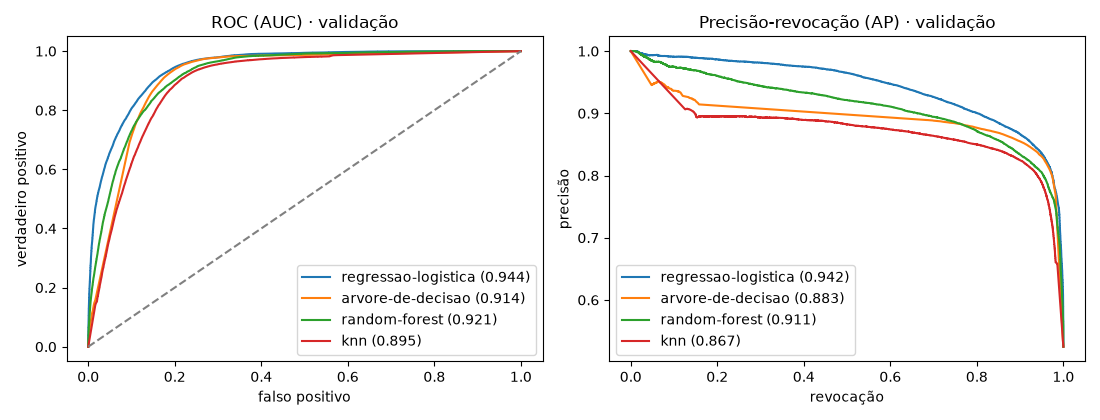
\includegraphics[width=.92\textwidth]{ml-01-roc-pr-comparacao.png}
\caption{Curvas ROC e de precisão-revocação dos quatro modelos com hiperparâmetros fixos, no conjunto
de validação.}
\label{fig:roc}
\end{figure}

Todos os modelos superam a lista fixa, por 2,4 a 5,4 pontos de F1-macro
(Tabela~\ref{tab:comparacao} e Figura~\ref{fig:roc}). Com hiperparâmetros fixos, a Regressão Logística
foi a melhor, a mais barata e a mais explicável. O KNN sobreajustou (0,984 no treino contra 0,846 na
validação) e é 60 vezes mais lento para prever, o que o descarta para a API. O Random Forest ficou
abaixo da árvore única, o que atribuímos a \texttt{max\_features="sqrt"}: com mais de 2.000 colunas
esparsas, cada divisão olhava só cerca de 2\% delas. Os quatro modelos erram juntos em 7,6\% das
palavras, em geral lemas ambíguos da Figura~\ref{fig:lemas}.

\subsection{Otimização e validação}

Escolhemos otimizar o Random Forest por ter mais hiperparâmetros e estar mais longe do seu limite. O
Optuna avaliou 25 configurações (número de árvores, profundidade, folhas mínimas, fração de atributos,
peso das classes e critério), cada uma com validação cruzada de 3 dobras numa amostra de 6.000 frases.
A melhor (154 árvores, profundidade 56, 3 exemplos por folha, 15\% dos atributos por divisão, classes
balanceadas, Gini) levou o F1-macro de validação de 0,852 para \textbf{0,884}, passando a Regressão
Logística. O ganho veio quase todo de \texttt{max\_features}, confirmando a hipótese acima, ao custo de
um treino 15 vezes mais lento (25 minutos).

\begin{figure}[ht]
\centering
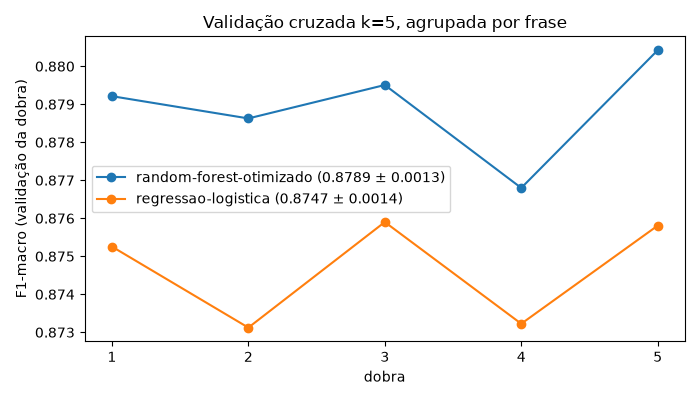
\includegraphics[width=.62\textwidth]{ml-05-cv-por-dobra.png}\\[4pt]
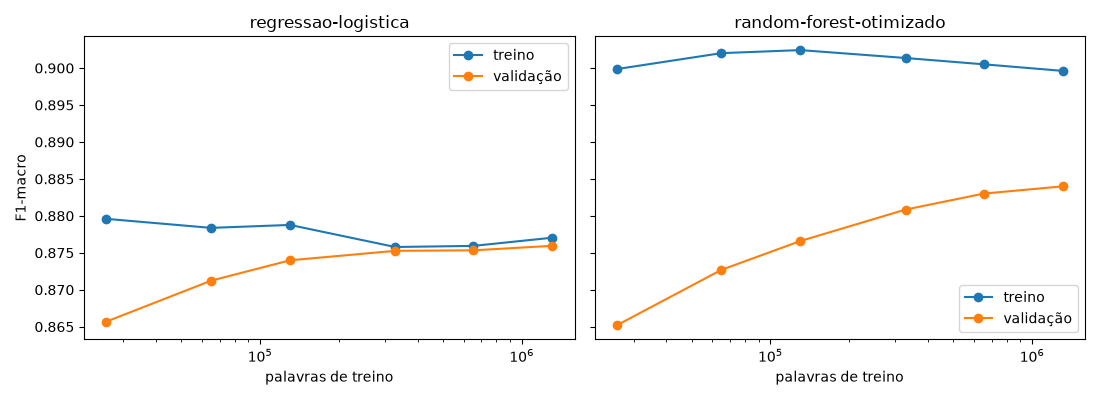
\includegraphics[width=\textwidth]{ml-06-curva-aprendizado.png}
\caption{Acima, F1-macro por dobra na validação cruzada agrupada por frase ($k=5$). Abaixo, curva de
aprendizado em treino e validação (eixo horizontal: palavras de treino, em escala logarítmica).}
\label{fig:cv}
\end{figure}

A validação cruzada (Figura~\ref{fig:cv}) mostra resultados \textbf{estáveis}: Random Forest otimizado
com 0,8789 $\pm$ 0,0013 e Regressão Logística com 0,8747 $\pm$ 0,0014; o Random Forest vence nas cinco
dobras, mas por apenas 0,4 ponto e sem vantagem em ROC-AUC. A curva de aprendizado indica
\textbf{subajuste leve} na Regressão Logística, que estaciona com 25\% dos dados (treino e validação
juntos em 0,876), e \textbf{sobreajuste moderado} no Random Forest, cuja diferença entre treino e
validação cai de 0,035 para 0,016 à medida que os dados crescem, com a validação ainda subindo. Fora
do domínio, os dois perdem de 2 a 4 pontos (a regressão perde menos), o que importa porque o produto
recebe textos de qualquer assunto.

\subsection{Teste final}

Pesando estabilidade, F1 e custo, o grupo escolheu o Random Forest otimizado. Ele foi treinado em todo
o conjunto de treino e avaliado uma única vez no teste (Tabela~\ref{tab:teste} e
Figura~\ref{fig:teste}).

\begin{table}[ht]
\centering
\caption{Conjunto de teste (10\% das frases, usado uma única vez).}
\label{tab:teste}
\begin{tabular}{lcc}
\hline
Métrica & Random Forest otimizado & Lista fixa (sem ML) \\
\hline
F1-macro                              & 0,885 & 0,823 \\
Acurácia                              & 0,886 & 0,826 \\
F1 \texttt{MANTER} / \texttt{DESCARTAR} & 0,896 / 0,874 & 0,848 / 0,797 \\
Revocação \texttt{DESCARTAR}          & 0,836 & 0,722 \\
ROC-AUC / PR-AUC                      & 0,947 / 0,941 & -- \\
\hline
\end{tabular}
\end{table}

\begin{figure}[ht]
\centering
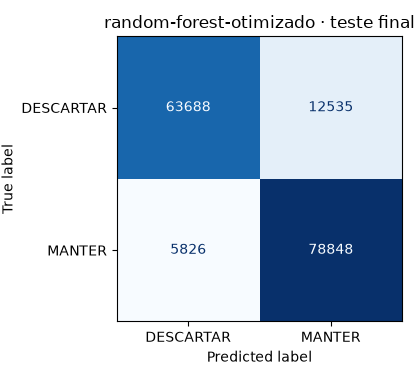
\includegraphics[width=.42\textwidth]{ml-08-matriz-confusao-teste.png}
\caption{Matriz de confusão do Random Forest otimizado no teste final (linhas: rótulo real; colunas: previsto).}
\label{fig:teste}
\end{figure}

O F1-macro de teste (0,885) coincide com o de validação (0,884) e com o da validação cruzada (0,879),
o que indica que não houve ajuste aos dados de validação. O ganho sobre a lista fixa se mantém:
\textbf{+6,2 pontos de F1-macro}. O erro mais comum é manter uma palavra que o intérprete descartou
(12.535 casos, contra 5.826 do erro oposto), coerente com o ruído assimétrico dos rótulos: parte
desses ``erros'' são palavras que o intérprete manteve com outra forma. O modelo foi registrado no
MLflow Model Registry como \texttt{sinaliza-t1}, versão 1, e é o que a API usa.

\section{Arquitetura e MLOps}\label{sec:mlops}

A Figura~\ref{fig:arquitetura} resume a solução. Os componentes de aprendizado de máquina nosso são o
treino e a inferência do T1; os demais são infraestrutura, regras ou serviços externos.

\begin{figure}[ht]
\centering
\resizebox{\textwidth}{!}{%
\begin{tikzpicture}[
  node distance=5mm and 6mm,
  box/.style={draw, rounded corners=2pt, align=center, font=\scriptsize, minimum height=8mm, minimum width=22mm, inner sep=3pt},
  ml/.style={box, line width=1.2pt},
  arr/.style={-{Latex[length=1.6mm]}, thin}]
\node[box] (corpus) {VLibrasBD\\(CSV)};
\node[box, right=of corpus] (ing) {Airflow\\ingestão e preparação};
\node[box, right=of ing] (pg1) {PostgreSQL\\\texttt{palavras\_t1}};
\node[ml, right=of pg1] (treino) {Airflow: treino,\\Optuna e validação};
\node[box, right=of treino] (mlflow) {MLflow: 4 experimentos\\e registro do modelo};
\node[box, below=10mm of corpus] (totem) {Totens simulados\\(embarcado)};
\node[box, right=of totem] (mqtt) {Broker MQTT\\(Mosquitto)};
\node[box, right=of mqtt] (rec) {Receptor\\\texttt{mensagens\_mqtt}};
\node[ml, right=of rec] (api) {API (FastAPI)\\classificador T1};
\node[box, right=of api] (avatar) {Sequência de sinais\\(player do VLibras)};
\node[box, below=10mm of rec] (web) {Front web\\(texto digitado)};
\node[box, below=10mm of avatar] (inf) {PostgreSQL\\\texttt{inferencias}};
\node[box, left=of inf] (mon) {Airflow\\monitoramento};
\node[box, below=5mm of mon] (painel) {Painel\\(Streamlit)};
\draw[arr] (corpus) -- (ing); \draw[arr] (ing) -- (pg1); \draw[arr] (pg1) -- (treino); \draw[arr] (treino) -- (mlflow);
\draw[arr] (mlflow.south west) -- node[left, font=\scriptsize, pos=.35]{\texttt{sinaliza-t1}} (api.north east);
\draw[arr] (totem) -- (mqtt); \draw[arr] (mqtt) -- (rec); \draw[arr] (rec) -- (api); \draw[arr] (api) -- (avatar);
\draw[arr] (web.north east) -- (api.south west);
\draw[arr] (api.south east) -- (inf.north west);
\draw[arr] (inf) -- (mon); \draw[arr] (mon) -- (painel);
\end{tikzpicture}}
\caption{Arquitetura do Sinaliza. Caixas com borda grossa são aprendizado de máquina nosso.}
\label{fig:arquitetura}
\end{figure}

\textbf{Aquisição e MQTT.} O sistema embarcado é \emph{simulado}: dois totens de atendimento (uma
unidade de saúde e uma agência do INSS) publicam frases públicas de atendimento no broker
Mosquitto~\cite{light:17}, no tópico \texttt{sinaliza/totens/<id>/frases}, com QoS 1, e o próprio estado
(online ou offline) num tópico retido com testamento (\emph{last will}). O receptor assina os tópicos,
grava cada mensagem no PostgreSQL \emph{antes} de pedir a inferência à API (assim nada se perde se a API
cair), ignora repetições pelo identificador da mensagem e tenta de novo até três vezes. Na pilha real,
cada frase levou de 0,2 a 0,7 segundo do totem até a inferência gravada; mensagens publicadas com o
receptor desligado chegaram quando ele voltou (sessão persistente), e um totem derrubado à força
apareceu offline em cerca de um segundo.

\textbf{Pipeline com Airflow.} Quatro DAGs~\cite{airflow:26} orquestram a ingestão, a preparação, o
treino (baseline, comparação, Optuna, validação cruzada e teste final, este protegido contra uma
segunda execução) e o monitoramento, que consolida a cada hora as inferências em indicadores. Numa
máquina sem dados, a primeira subida roda sozinha ingestão, preparação e treino.

\textbf{Rastreamento com MLflow.} Cada etapa tem seu próprio experimento~\cite{zaharia:18}: baseline
(2 runs), comparação de modelos (4), otimização de hiperparâmetros (a run do estudo, 25 tentativas filhas
e o modelo otimizado) e validação com teste final (6), numerados de \texttt{sinaliza-t1-01-baseline} a
\texttt{sinaliza-t1-04-validacao-e-teste-final}. Todas as runs registram parâmetros, métricas, artefatos
(matrizes de confusão, curvas, importâncias, tabelas) e o modelo salvo.

\textbf{API e integração.} A API (FastAPI) carrega o \texttt{sinaliza-t1} do registro do MLflow e, a
cada frase, devolve a decisão e a probabilidade de cada palavra, a sequência de sinais e a versão do
modelo, com latência mediana de cerca de 180~ms. As frases vindas do simulador ou dos totens são
gravadas e consumidas automaticamente pelo DAG de monitoramento.

\textbf{Painel.} O painel em Streamlit mostra frases e latência por hora, proporção de palavras
mantidas, decisões incertas (probabilidade entre 0,4 e 0,6), palavras sem sinal no vocabulário, as
últimas inferências palavra por palavra, os totens (online, mensagens, latência ponta a ponta e
mensagens perdidas pela numeração), a versão e as métricas do modelo e o estado de cada serviço.

\textbf{Docker.} Um único \texttt{docker compose up -d -{}-build} sobe os dez serviços (PostgreSQL,
MLflow, API, Airflow, painel, front web, broker MQTT, receptor e dois totens) na ordem certa, em cerca de
2,7~GB de memória. Uma demonstração automática percorre as oito etapas do fluxo e passou em todas.

\section{Limitações}\label{sec:limitacoes}

\begin{itemize}
\item A saída é uma sequência de sinais na ordem do português; o modelo não trata gramática nem
  ordem da Libras, e nada foi validado por pessoas surdas ou intérpretes.
\item Os rótulos vêm de uma regra com cerca de 8\% de erro, concentrado em \texttt{DESCARTAR}; o F1
  medido é proximidade às glosas, não correção linguística.
\item A generalização para outros assuntos é fraca (queda de 2 a 4 pontos fora do domínio), e o
  modelo foi treinado em frases isoladas, enquanto a API recebe textos que podem ter várias frases.
\item O modelo escolhido exige cerca de 2,8~GB na carga e 25 minutos de treino; a Regressão Logística
  seria uma alternativa mais leve com só 0,4 ponto a menos.
\item O sistema embarcado é simulado e o broker roda sem autenticação nem TLS, adequado só ao uso
  local.
\end{itemize}

\section{Conclusão}\label{sec:conclusao}

Mostramos que a decisão de quais palavras viram sinal pode ser aprendida das glosas de intérpretes: o
Random Forest otimizado chegou a F1-macro de 0,885 no teste, 6,2 pontos acima da lista fixa, com
resultados estáveis na validação cruzada agrupada por frase. O ganho está onde a análise exploratória
indicava: nas classes gramaticais intermediárias e nos lemas ambíguos, em que o contexto decide. A
solução roda de ponta a ponta com aquisição simulada via MQTT, orquestração no Airflow, rastreamento
no MLflow, inferência pela API e monitoramento no painel, tudo reproduzível com um comando. Os
próximos passos são melhorar a rotulagem (comparação por radical e normalização de números), tratar
textos com várias frases e, principalmente, avaliar a saída com pessoas surdas.

\bibliographystyle{sbc}
\bibliography{referencias}

\end{document}
